%%%%%%%%%%%%%%%%%%%%%%%%%%%%%%%%%%%%%%%%%%%%%%%%%%%
%                                                 %
%                     SECTION                     %
%                                                 %
%%%%%%%%%%%%%%%%%%%%%%%%%%%%%%%%%%%%%%%%%%%%%%%%%%%

\section{Methodology}
\label{sec:sec003}

The hereby used prototypes are both \hyperlink{https://github.com/mida-project/prototype-multi-modality-assistant/releases/tag/v1.2.0-alpha}{v1.2.0-alpha} and \hyperlink{https://github.com/mida-project/prototype-heatmap/releases/tag/v1.2.0-alpha}{v1.2.0-alpha} versions of our {\it \hyperlink{https://github.com/mida-project/prototype-multi-modality-assistant/}{Assistant}} and {\it \hyperlink{https://github.com/mida-project/prototype-heatmap}{Heatpmap}} prototypes, respectively. The purpose of these prototypes is to involve an \textit{AI-Assisted} tool (\textit{Assistant}) for medical imaging at a breast screening diagnosis level. This \textit{Assistant} was created with a front-end and back-end architecture utilizing common programming languages, libraries, frameworks and tools including \hyperlink{https://www.javascript.com/}{JavaScript (JS)}~\cite{flanagan2006javascript}, \hyperlink{https://nodejs.org/}{NodeJS}~\cite{wilson2018node}, \hyperlink{https://hammerjs.github.io/}{HammerJS}, \hyperlink{https://cornerstonejs.org/}{CornerstoneJS}~\cite{hostetter2018integration} and \hyperlink{https://www.orthanc-server.com/}{Orthanc}~\cite{Jodogne:ISBI2013}. For the Machine Learning (ML) and Deep Learning (DL)~\cite{ribeiro2017real, ribeiro2016real} component we will use several \hyperlink{https://www.mathworks.com/products/matlab.html}{MATLAB} technologies~\cite{vedaldi2015matconvnet}, promoting and feeding our Convolutional Neural Networks (CNN)~\cite{carneiro2015unregistered} and Deep Reenforcement Learning (DRL)~\cite{maicas2017deep} techniques. Other central component of this prototype is a web-based \hyperlink{https://www.sciencedirect.com/topics/medicine-and-dentistry/picture-archiving-and-communication-system}{PACS}~\cite{cooke2003picture} pairwise with ubicous web technologies and based on the \textbf{Open Source (OS)} \hyperlink{https://cornerstonejs.org/}{CornerstoneJS} library~\cite{feller2002understanding, hostetter2018integration}.

%%%%%%%%%%%%%%%%%%%%%%%%%%%%%%%%%%%%%%%%%%%%%%%%%%%
%                                                 %
%                     SECTION                     %
%                                                 %
%%%%%%%%%%%%%%%%%%%%%%%%%%%%%%%%%%%%%%%%%%%%%%%%%%%

\subsection{Environments}

This section describes the user environment over interaction, the so called \textbf{Radiology Room (RR)} (Figure \ref{fig:radioroom}). This guide is based on soft-copy diagnosis using computer workstations in their current reading room environment. It will be here where we take impressions regarding the efficacy of radiologists, and their recommendations based on their experience for improvements on the soft-copy reading environment. Several studies demonstrated~\cite{waite2017tired} that radiologist fatigue levels and performance are related to environmental factors such as number of False-Negative (FN) and False-Positives (FP), in addition to workstation enhancements. Supported by this guide, our research aims to conduct an investigation for the several environmental variables and improvements regarding the potentially enhancement that an \textit{AI-Assisted} diagnosis could take in the \textbf{RR}.

%%%%%%%%%%%%%%%%%%%%%%%%%%%%%%%%%%%%%%%%%%%%%%%%%%%

\begin{figure}[h]
\centering
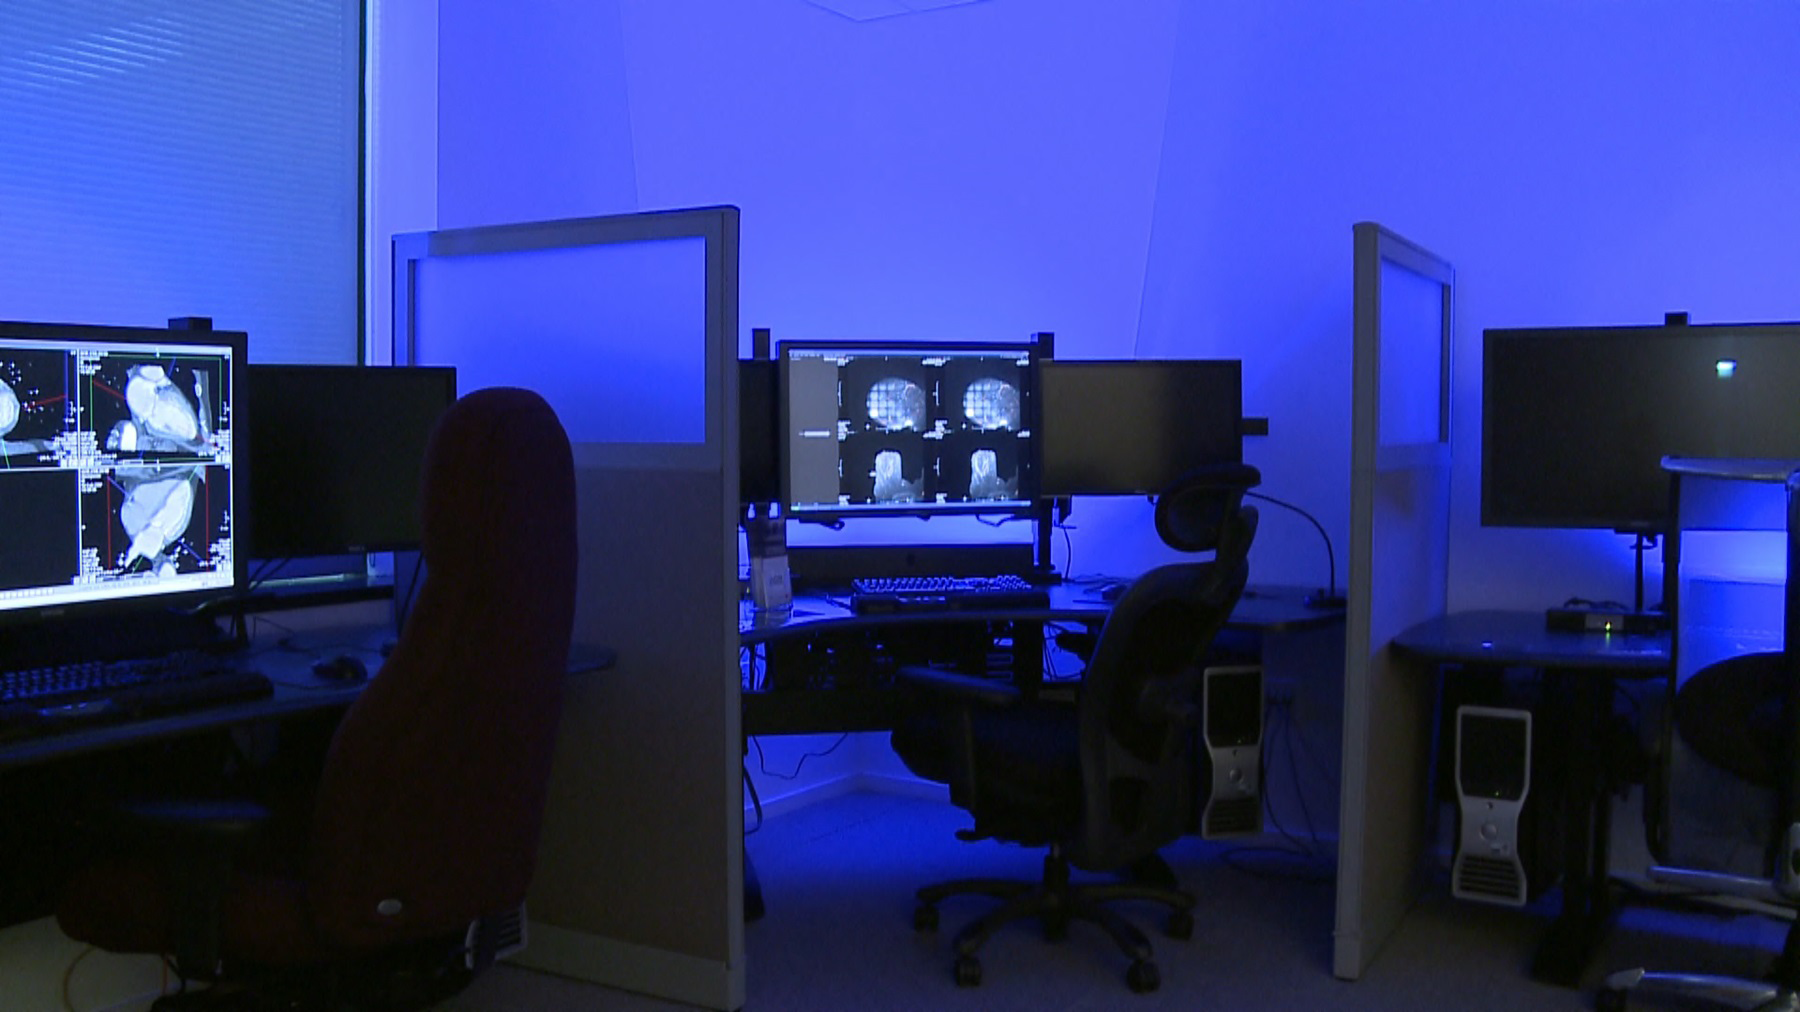
\includegraphics[width=\textwidth]{acr}
\caption{Radiology Room}
\label{fig:radioroom}
\end{figure}

%%%%%%%%%%%%%%%%%%%%%%%%%%%%%%%%%%%%%%%%%%%%%%%%%%%

%%%%%%%%%%%%%%%%%%%%%%%%%%%%%%%%%%%%%%%%%%%%%%%%%%%
%                                                 %
%                     SECTION                     %
%                                                 %
%%%%%%%%%%%%%%%%%%%%%%%%%%%%%%%%%%%%%%%%%%%%%%%%%%%

\subsection{Participants}

The participants' responsibilities will be attempting to complete a set of representative task scenarios (Section \ref{sec:sec007}) presented to them in as efficient and timely a manner as possible, and to provide feedback regarding the usability and acceptability of an \textit{AI-Assisted} diagnosis. The participants will be directed to provide honest opinions regarding the user tests of the interacted systems, and to participate in post-session subjective questionnaires and debriefing.

%%%%%%%%%%%%%%%%%%%%%%%%%%%%%%%%%%%%%%%%%%%%%%%%%%%

%%%%%%%%%%%%%%%%%%%%%%%%%%%%%%%%%%%%%%%%%%%%%%%%%%%
%                                                 %
%                     SECTION                     %
%                                                 %
%%%%%%%%%%%%%%%%%%%%%%%%%%%%%%%%%%%%%%%%%%%%%%%%%%%

\subsection{Procedure}

Participants will take part in the tests at our formed institution protocols (\textit{e.g.}, \hyperlink{http://hff.min-saude.pt/}{Hospital Fernando Fonseca (HFF)}) with both \hyperlink{https://github.com/mida-project/prototype-multi-modality-assistant/releases/tag/v1.2.0-alpha}{v1.2.0-alpha} and \hyperlink{https://github.com/mida-project/prototype-heatmap/releases/tag/v1.2.0-alpha}{v1.2.0-alpha} versions of our \hyperlink{https://github.com/mida-project/prototype-multi-modality-assistant/}{prototype-multi-modality-assistant} and \hyperlink{https://github.com/mida-project/prototype-heatmap}{prototype-heatmap} repositories, respectively. The interaction with the system will be used in a typical \textbf{RR} environment. Note takers and data logger(s) will monitor the sessions for observation in the \textbf{RR}, connected by screen recording feed. The test sessions will be recorded and further analyzed.

The facilitator will brief the participants on the system features and instruct the participant that they are evaluating the system, rather than the facilitator evaluating the participant. Participants will sign an informed consent (\textbf{Pha1.} - \textbf{Act1.}) that acknowledges: the participation is voluntary, that participation can cease at any time, and that the session will be videotaped and eye tracked but their privacy of identification will be safeguarded. The facilitator will ask the participant if they have any questions.

\hfill

Participants will complete a pre-test demographic (\textbf{Pha1.} - \textbf{Act3.}) and background information (\textbf{Pha1.} - \textbf{Act2.}) questionnaires. The facilitator will explain that the amount of time taken to complete the test task, will be measured and that exploratory behavior outside the task flow should not occur until after task completion. At the start of each task, the participant will listen the task description from the printed copy and begin the task. Time-on-Task (ToT) measurement~\cite{reale2018using} begins when the participant starts the task.

The facilitator will instruct the participant to "think aloud"~\cite{bolle2016authors, kilsdonk2016uncovering} so that a verbal record exists of their interaction with the system. The facilitator will observe and enter user behavior, user comments, and system actions. Before each task, participants will complete a pre-task (\textbf{Pha2.} - \textbf{Act8.}) questionnaire. During each task, participants will elaborate on the task session (\textbf{Pha2.} - \textbf{Act5.} and \textbf{Act6.}) and complete the post-task (\textbf{Pha2.} - \textbf{Act7.}) questionnaires with the facilitator. After all task scenarios are attempted, the participant will complete several {\it \hyperlink{https://www.nngroup.com/articles/open-ended-questions/}{open-ended questions}}~\cite{abelson2016supporting, merchant2018digital}.

%%%%%%%%%%%%%%%%%%%%%%%%%%%%%%%%%%%%%%%%%%%%%%%%%%%

%%%%%%%%%%%%%%%%%%%%%%%%%%%%%%%%%%%%%%%%%%%%%%%%%%%
%                                                 %
%                     SECTION                     %
%                                                 %
%%%%%%%%%%%%%%%%%%%%%%%%%%%%%%%%%%%%%%%%%%%%%%%%%%%

\subsection{Briefing}

A presentation of the \textit{Assistant} and its use and capabilities will be made. Participants will be presented to the available interactions and will be explained how to interact with the prototype, underlining the limitations. The facilitator will brief the participants on the \textit{Assistant} system and instruct the participant that they are evaluating the system, rather than the facilitator evaluating the participant. Participants will sign an informed consent that acknowledges: the participation is voluntary, that participation can cease at any time, and that the session will be videotaped and eye gaze monitorization but their privacy of identification will be granted. The facilitator will ask the participant if they have any question.

%%%%%%%%%%%%%%%%%%%%%%%%%%%%%%%%%%%%%%%%%%%%%%%%%%%

%%%%%%%%%%%%%%%%%%%%%%%%%%%%%%%%%%%%%%%%%%%%%%%%%%%
%                                                 %
%                     SECTION                     %
%                                                 %
%%%%%%%%%%%%%%%%%%%%%%%%%%%%%%%%%%%%%%%%%%%%%%%%%%%

\subsection{Training}

The participants will receive and overview of the user test procedure, equipment and system. The facilitator will show how to interact with the system and what features are available. We choose this approach, as it provide clinicians the most important concepts to understand and interact with our system. Also, it is of chief importance to give clinicians information of what is and is not available analysis of our \textit{Assistant} and what it can do.

%%%%%%%%%%%%%%%%%%%%%%%%%%%%%%%%%%%%%%%%%%%%%%%%%%%

\clearpage